\documentclass[10pt,a4paper]{article}
\usepackage[margin=2.3cm]{geometry}
\usepackage{amsmath,amssymb}
\usepackage{booktabs,array,longtable,tabularx}
\usepackage{graphicx,float,caption}
\usepackage{xcolor}
\usepackage{listings}
\usepackage{enumitem}
\usepackage{tikz}
\usetikzlibrary{arrows.meta,positioning,calc}
\usepackage[colorlinks=true,linkcolor=teal!50!black,urlcolor=blue!50!black,citecolor=teal!50!black]{hyperref}
\usepackage{microtype}
\usepackage{seqsplit}
\emergencystretch=2em

\setlist{itemsep=2pt,topsep=3pt,parsep=0pt}
\captionsetup{font=small,labelfont=bf}
\setlength{\parindent}{0pt}
\setlength{\parskip}{5pt}
\renewcommand{\arraystretch}{1.12}

\definecolor{cgood}{HTML}{0F766E}
\definecolor{cbad}{HTML}{C2410C}
\lstset{basicstyle=\ttfamily\footnotesize,breaklines=true,frame=single,rulecolor=\color{black!25},
        backgroundcolor=\color{black!3},columns=fullflexible,keepspaces=true,showstringspaces=false}

\newcommand{\tx}[1]{\texttt{\detokenize{#1}}}
\newcommand{\txl}[1]{\texttt{\expandafter\seqsplit\expandafter{\detokenize{#1}}}}
\newcommand{\KLD}{\mathrm{KLD}}
\newcommand{\W}{\mathbf{W}}
\newcommand{\X}{\mathbf{x}}
\newcommand{\HD}{\mathbf{R}}

\title{\textbf{Q4-quality, 8k-prefill INT4 inference for Ossicle-4B on RDNA3}\\[2pt]
\large Rotated GPTQ weights, 8-bit and 4-bit activations on WMMA, and what it cost\\[-2pt]
\normalsize A technical report on the full run: methods, measurements, failures}
\author{Work log compiled from the session logs, scripts and commits}
\date{1 November 2026}

\begin{document}
\maketitle
\thispagestyle{empty}

\begin{abstract}
\noindent
We take the Ossicle-4B audio--language model (Qwen3.5-4B backbone, Qwen3-Omni AuT audio encoder), convert it to GGUF for
llama.cpp, quantise it in ten standard formats, and then build a custom prefill/decode path for a single AMD RX~7900~XT
(RDNA3, \tx{gfx1100}) that stores every linear weight \emph{Hadamard-rotated}, \emph{GPTQ-quantised} to symmetric int4, and
multiplies it on the int4 WMMA units against rotated 8-bit or 4-bit activations.
The shipped file (2.55\,GB) reaches \textbf{5{,}846 tokens/s prefill (pp512) at KLD~0.025 against BF16} with decode at
131.8\,tokens/s, i.e.\ better agreement with BF16 than Q4\_K\_M (KLD~0.030--0.032) and about 24\% faster prefill.
A one-variable preset, \tx{GGML_INT4_PREFILL=fast}, raises prefill to \textbf{8{,}269\,tokens/s (pp2048: 7{,}802) with decode
unchanged at 131.7\,tokens/s}, at KLD~0.096 (Q4\_0--Q3\_K\_L class by KLD, MMAU unchanged within noise).
We document every experiment, including the ones that failed (a chunked gated-delta-net kernel, FP4 re-gridding, sparsity
skipping, wider weight scale groups) and the caveats that remain.
\end{abstract}

\vspace{4pt}
\begin{center}
\small
\begin{tabular}{@{}lrrrrrr@{}}
\toprule
\textbf{Headline (RX 7900 XT, ROCm 10.1.0)} & pp512 & pp2048 & tg128 & KLD & same top-1 & MMAU\\
\midrule
Q4\_K\_M (best stock Q4, reference) & 4{,}733 & 4{,}595 & 131.6 & 0.032 & 91\% & 72.2\\
rotated INT4, \tx{quality} (default) & 5{,}846 & 5{,}647 & 131.8 & 0.025 & 92.5\% & 71.7\\
rotated INT4, \tx{balanced} & 7{,}257 & 6{,}935 & 131.5 & 0.071 & 87.3\% & --\\
rotated INT4, \tx{fast} & \textbf{8{,}269} & \textbf{7{,}802} & 131.7 & 0.096 & 85.4\% & 71.6\\
\bottomrule
\end{tabular}
\end{center}

\tableofcontents
\newpage

%=====================================================================================================================
\section{Goal, hardware and model}
\label{sec:goal}

The work proceeded in a sequence of requests, each building on the last:
\begin{enumerate}
\item Convert the BF16 Ossicle-4B checkpoint to GGUF; quantise it in the usual llama.cpp formats; measure quality (perplexity,
      KL divergence, MMAU) and speed on an RX~7900~XT and an RTX~5060~Ti; push the result to a private HF repository.
\item Fix the audio front end of llama.cpp so GGUF accuracy matches PyTorch (opt-in GGUF keys), and move AMD to ROCm~10.1.
\item Use the 7900~XT's int4 matrix instructions for a faster prefill (a ``W4A4'' path).
\item \emph{``Get decode up and reduce KL vs BF16. Get it to Q4 quality.''}
\item \emph{``Get me 8k prefill with this decode.''}
\end{enumerate}
Items 4 and 5 are the focus of this report; items 1--3 are summarised (Sections~\ref{sec:baseline}--\ref{sec:wmma}) because
the later work depends on them.

\paragraph{Hardware and software.}
GPU: AMD Radeon RX~7900~XT (gfx1100, wave32, 20\,GB, 254\,W power cap, sustained clock $\approx$2.28\,GHz).
Second GPU for cross-checking the standard quants: NVIDIA RTX~5060~Ti 16\,GB (CUDA~13.0).
ROCm~10.1.0 from the pip wheels (isolated venv; ROCm~7.2.0 kept for comparison). llama.cpp fork
\tx{SILVERTHRONE32/llama.cpp-ossicle}, branch \tx{ossicle}, based on upstream \tx{f2b52a87e}; current head \tx{1fcc55e87}.

\paragraph{Model.}
The language model is Qwen3.5-4B (merged LoRA), 4.21\,B parameters: 32 layers, hidden size 2560, FFN width 9216, vocabulary
248{,}320 with tied embedding/head (1.27\,GB in BF16). Layers alternate three \emph{gated-delta-net} (GDN, linear-attention)
layers with one full-attention layer (24 GDN + 8 attention). GDN uses 16 key heads, 32 value heads, head dimension 128 and a
4-wide causal convolution; full attention uses 16 query heads, 4 KV heads, head dimension 256.
The 200 quantised linear tensors are, per layer kind: GDN \tx{attn_qkv}, \tx{attn_gate} (the z-gate), \tx{ssm_out}; attention
\tx{attn_q}, \tx{attn_k}, \tx{attn_v}, \tx{attn_output}; and in every layer \tx{ffn_gate}, \tx{ffn_up}, \tx{ffn_down}
($24\!\times\!3+8\!\times\!4+32\!\times\!3=200$).

\paragraph{Metrics.}
\begin{itemize}
\item \textbf{KLD / same-top-1}: \tx{llama-perplexity --kl-divergence} against logits of the BF16 GGUF on WikiText-2 test, context 512,
      24 chunks ($\approx$12k tokens). Standard error is about $\pm0.001$ near KLD~0.025 and $\pm0.003$ near 0.1.
\item \textbf{PPL}: WikiText-2 test, full set (standard quants) or the same 24 chunks (INT4 variants; stated as ``vs BF16'').
\item \textbf{MMAU}: test-mini, 1000 questions, greedy decoding through \tx{llama-server}, string-match scorer; standard error
      $\pm$1.4\,pp, so differences under $\sim$3\,pp are noise. PyTorch BF16 scores 72.1.
\item \textbf{Speed}: \tx{llama-bench}. For the INT4 work we use the \emph{median of 8 runs after discarding the first}
      (\txl{scripts/bench_med.sh}: \tx{-r 9}, first sample dropped), because the first sample is taken at cold GPU clocks and
      wrecks short means (e.g.\ one 3-run bench logged pp512 $4810\pm1416$ against a steady 5{,}846).
\end{itemize}

%=====================================================================================================================
\section{Baseline: GGUF conversion and the standard quant ladder}
\label{sec:baseline}

The BF16 safetensors were converted with llama.cpp's \tx{qwen35} text architecture and \tx{qwen3a} mmproj
(\txl{scripts/convert_ossicle.py}); the chat template is patched to always emit an empty \tx{<think>} block, which is how
Ossicle was trained. Ten quants were produced with an importance matrix from WikiText-2 train (Q8\_0 without) and each was
measured on both GPUs. Table~\ref{tab:quants} is the quality table, Table~\ref{tab:quantspeed} the speed table.

\begin{table}[H]
\centering\small
\caption{Standard quants of Ossicle-4B. PPL: WikiText-2 test. MMAU: patched llama.cpp (audio fix of Section~\ref{sec:audio}).}
\label{tab:quants}
\begin{tabular}{@{}lrrrrrrr@{}}
\toprule
Quant & GB & PPL & KLD & top-1 \% & MMAU XT & MMAU Ti & MMAU stock\\
\midrule
BF16 (ref) & 8.42 & 10.571 & -- & -- & 71.8 & 71.8 & 70.2\\
Q8\_0 & 4.48 & 10.566 & 0.0023 & 97.9 & 72.3 & 72.1 & 70.5\\
Q6\_K & 3.46 & 10.670 & 0.0063 & 95.6 & 72.3 & 72.4 & 70.5\\
Q5\_K\_M & 3.08 & 10.740 & 0.0146 & 94.0 & 72.8 & 72.2 & 71.2\\
Q4\_K\_M & 2.71 & 10.951 & 0.0303 & 91.1 & 72.1 & 72.4 & 70.0\\
Q4\_K\_S & 2.56 & 10.939 & 0.0346 & 90.8 & 72.0 & 71.9 & 70.8\\
Q4\_0 & 2.55 & 10.994 & 0.0581 & 89.2 & 71.9 & 71.7 & 70.8\\
IQ4\_XS & 2.51 & 10.884 & 0.0346 & 90.9 & 72.0 & 71.4 & 70.9\\
Q3\_K\_L & 2.42 & 11.681 & 0.1011 & 85.5 & 70.3 & 70.2 & 69.4\\
Q3\_K\_M & 2.26 & 11.820 & 0.1077 & 85.0 & 70.6 & 70.7 & 70.5\\
Q3\_K\_S & 2.07 & 12.203 & 0.1492 & 82.5 & 69.6 & 69.9 & 69.3\\
\bottomrule
\end{tabular}
\end{table}

\begin{table}[H]
\centering\small
\caption{Speed of the standard quants (first-token = full \tx{llama-server} path with one 10\,s clip; XT = 7900~XT/ROCm 10.1,
Ti = 5060~Ti/CUDA 13.0). These use a different method from the INT4 tables (server median of 5), hence Q4\_K\_M pp512 of 4{,}482
here against 4{,}733 in the INT4 comparisons.}
\label{tab:quantspeed}
\begin{tabular}{@{}lrrrrrr@{}}
\toprule
Quant & XT pp512 & XT first tok (ms) & XT tg (t/s) & Ti pp512 & Ti first tok (ms) & Ti tg (t/s)\\
\midrule
BF16 & -- & -- & -- & 3933 & 167 & 47.0\\
Q8\_0 & 4775 & 150 & 95.4 & 4971 & 139 & 81.2\\
Q6\_K & 4035 & 170 & 115.7 & 4141 & 136 & 98.6\\
Q5\_K\_M & 4484 & 150 & 120.2 & 4572 & 130 & 108.1\\
Q4\_K\_M & 4482 & 153 & 126.6 & 4653 & 128 & 119.0\\
Q4\_K\_S & 4552 & 144 & 129.5 & 4802 & 128 & 124.3\\
Q4\_0 & 4602 & 149 & 130.7 & 5033 & 121 & 128.5\\
IQ4\_XS & 4675 & 144 & 136.5 & 5035 & 122 & 127.9\\
Q3\_K\_L & 4109 & 152 & 127.7 & 4448 & 131 & 118.2\\
Q3\_K\_M & 4118 & 150 & 131.1 & 4441 & 129 & 123.3\\
Q3\_K\_S & 3905 & 154 & 132.8 & 4206 & 131 & 123.8\\
\bottomrule
\end{tabular}
\end{table}

Observations that shaped later decisions:
\begin{itemize}
\item KLD orders the quants cleanly; MMAU between Q8\_0 and IQ4\_XS (71.4--72.8) is inside noise, and only the Q3 family drops
      below the PyTorch reference. We therefore use KLD for ranking and MMAU as a sanity check.
\item Q4\_K\_M's prefill (about 4.5--4.7k t/s) is the number to beat; the llama.cpp INT8 MMQ path tops out near
      36--40 TOPS on this card.
\item Mixed-precision storage is cheap: the 1.27\,GB BF16 token-embedding/head tensor alone costs about 1\,ms per decoded
      token (Section~\ref{sec:decode}).
\end{itemize}

%=====================================================================================================================
\section{Audio front-end fix and ROCm 10.1}
\label{sec:audio}

\paragraph{Audio.} On stock llama.cpp the BF16 GGUF scores 70.2 on MMAU against 72.1 for PyTorch. Three differences in
the mtmd audio path were found and fixed as \emph{opt-in} GGUF keys (default off, so other models behave as upstream):
\txl{clip.audio.no_boundary_tokens} (Ossicle never saw \tx{<|audio_start|>}/\tx{<|audio_end|>}; $\approx$+1.2\,pp),
\txl{clip.audio.polyphase_resample} (Kaiser polyphase like \txl{scipy.signal.resample_poly} instead of linear; $\approx$+0.7\,pp)
and \txl{clip.audio.exact_frame_count} (\texttt{ceil(n/hop)} mel frames as \txl{WhisperFeatureExtractor}; $\approx$+0.3\,pp).
Patched BF16 reaches 71.8 (976/1000 answers identical to PyTorch). As a transfer check, the same two applicable keys lifted
Qwen3-Omni-30B-A3B (Q4\_K\_M) from 78.9 to 80.0 MMAU (+1.10$\pm$0.46\,pp paired, 16 up/5 down).

\paragraph{ROCm.} On ROCm~7.2.0, Q8\_0 and IQ4\_XS (pp512 $\approx$1{,}100--1{,}300) and short-batch Q4\_0 had slow
prefill; ROCm~10.1.0 fixes it (Q8\_0 pp512 1{,}123\,$\to$\,4{,}775) at the price of 1--3\% slower generation. All later work
uses 10.1.0.

%=====================================================================================================================
\section{Int4 WMMA microbenchmarks}
\label{sec:wmma}

RDNA3 exposes \texttt{v\_wmma\_i32\_16x16x16\_iu4} at \emph{twice} the rate of the iu8 variant. A pure-WMMA
microbenchmark sustains 182~TOPS (190 on paper; about 195 at the 2.28\,GHz this card holds at its power cap).

A standalone kernel was developed through 27 successive variants (\txl{kernel/q4k_iu4_v2} \ldots\ \txl{q4s_iu4_v27}), always
verified against a CPU reference (relative error $4.5\!\times\!10^{-4}$). The format: symmetric int4 weights (signed codes,
no zero point) with one integer sub-scale per 32/64/128 K-values, multiplied by int4 activations.

\begin{table}[H]
\centering\small
\caption{Standalone int4 GEMM throughput after warm-up (FFN $9216\times2560$ at $N=512$; down $2560\times9216$ at $N=2048$).}
\begin{tabular}{@{}lrrrr@{}}
\toprule
Sub-scale per & FFN $N{=}512$ & FFN $N{=}2048$ & down $N{=}2048$ & extra KLD vs per-32\\
\midrule
32 K-values & 125 TOPS & 128 & 124 & --\\
64 & 142 & 144 & 143 & +0.011\\
128 & \textbf{149} & \textbf{149} & \textbf{152} & +0.015\\
\bottomrule
\end{tabular}
\end{table}
That is 78\% of the sustained theoretical peak and 83\% of the best pure-WMMA loop. Where the rest goes: fragment loads
$\approx$8--10\%, integer scaling $\approx$5\%, loop structure $\approx$4\%. At llama.cpp's own reference shape
(Q4\_K, $M{=}4096$, $N{=}512$, $K{=}14336$) the pipeline ``fused Hadamard rotation + quantise (0.04\,ms) + GEMM (0.43\,ms)''
takes 0.47\,ms (128 TOPS end-to-end) against 1.52\,ms (39.6 TFLOPS in \tx{test-backend-ops}) for the existing INT8 MMQ,
i.e.\ about 3.2$\times$ on the matmul.

What got there: operand-ready weight repacking; scalar buffer-load addressing; 24-bit integer multiply-adds (inline asm);
8+ independent WMMA chains with scheduler barriers; chaining the accumulator through a whole scale unit (one multiply-add per
unit); arranging a block's waves along the token dimension (1$\times$8 waves so the weight tile is shared through cache);
and a fused one-pass rotate+quantise+pack kernel (HadaCore idea, own RDNA3 implementation).

\paragraph{Benchmark pitfall.} With only $\sim$10\,ms of launches the GPU never reaches full clocks and a kernel looks about
1.5$\times$ slower (71 vs 110 TOPS for the same kernel). Warm up for at least 1\,s of load. The same effect is why the
\tx{llama-bench} medians drop the first sample.

\paragraph{Dead ends in the microbenchmark phase.}
\begin{itemize}
\item \textbf{FP4 checkpoints.} E2M1 needs 5 bits once doubled, so it cannot go through one int4 pass exactly. Re-fitting
      NVFP4/MXFP4 weights onto a uniform int4 grid cost about +0.07 KLD (0.096 native $\to$ 0.16--0.19). Plain symmetric int4
      from a BF16 source is as accurate as FP4 (0.082 vs 0.098).
\item \textbf{Sparsity skipping.} A wave-uniform group-skip loop is exact (62\,$\to$\,98 TOPS at 75\% skipped) but real
      activations give almost nothing to skip: all-zero 16-token$\times$32-value tiles are 0--0.3\% lossless and 2--6\% even
      under aggressive thresholds (\txl{int4/sparsity_probe*.py}).
\end{itemize}

%=====================================================================================================================
\section{The rotated-INT4 format}
\label{sec:format}

\subsection{Rotation}
Four-bit \emph{activations} are the quality risk: transformer activations have outlier channels. We rotate with a
block-Hadamard transform. For a linear layer $y=\W\X$ with input dimension $K$ (multiple of 256), define per 256-block
\[
  \HD = \tfrac{1}{16}\,H_{256}\,D,\qquad D=\mathrm{diag}(s_j),\quad s_j=-1\ \text{if}\ \big((j\cdot 2654435761)\bmod 2^{32}\big)\gg 31,\ \text{else}\ +1,
\]
where $H_{256}$ is the Sylvester Hadamard matrix. $\HD$ is orthogonal, so $\W'=\W\HD^{\!\top}$ (applied blockwise along $K$) and
$\X'=\HD\X$ give $\W'\X'=\W\X$ exactly. The weights are rotated \emph{offline} (\tx{scripts/rotate_quantize.py}); activations
are rotated \emph{online} in the backend. The sign pattern is a hash so the C++ side and the converter agree without storing it.
Rotation Gaussianises both operands, which is what makes 4-bit codes viable.

\subsection{GPTQ on the rotated weights}
The initial files used round-to-nearest (RTN) with $|\max|/7$ scales and codes in $[-7,7]$. The final files use GPTQ
(\tx{scripts/gptq_rotate.py}):
\begin{enumerate}
\item Load the Ossicle LM in transformers (from \tx{stage_lm} and the \tx{src/} safetensors), BF16 on GPU.
\item Register a forward pre-hook on each of the 200 target linears; for the rotated input $\X'$ (in llama.cpp column order,
      including the out-projection head re-order) accumulate $H=\sum \X'^{\!\top}\X'$ in fp32 on the CPU.
      Calibration: 128 sequences $\times$ 512 tokens of WikiText-2 \emph{train}, batches of 8.
\item For each tensor, GPTQ with Cholesky-inverse error feedback (damping 0.01 of the mean diagonal, column blocks of 128),
      codes in $[-8,7]$, one fp16 scale per group of 32 columns. Each group's scale is chosen on the error-compensated
      weights by an MSE search over 26 candidates $\{0.55,\ldots,1.05\}\cdot\max|w|/7$, rounded to fp16.
\item Pack as ordinary \textbf{Q4\_0 blocks} (fp16 scale + 16 bytes: element $j$ low nibble, $j{+}16$ high nibble) in a
      safetensors file keyed by GGUF tensor name. No new GGUF type is introduced.
\item \tx{rotate_quantize.py --blocks} rebuilds the GGUF from BF16, re-rotating each tensor and \emph{asserting the dequantised
      blocks are within 0.25 relative error of it} (a wrong row/column order shows up as $\approx$1.0).
\end{enumerate}
GPTQ runs end-to-end in about four minutes (Hessians + 200 tensors; the quantisation loop itself $\approx$106\,s) and
about 15\,GB of RAM. Mean relative weight error: 0.1071 (group 32), 0.1179 (group 64). A group-128 run died with ENOSPC (see
Section~\ref{sec:errors}) and was dropped.

The token embedding/output head is requantised separately: Q6\_K (via \tx{ggml_quantize_chunk}) or Q8\_0. The GGUF gains two keys,
\txl{ossicle.int4_rotation_block}=256 and \txl{ossicle.int4_scale_group}; the loader sets \tx{GGML_INT4=3} automatically when
the first is present.

\subsection{How much does each ingredient buy?}
Because iterating on the real runtime is slow, a Hugging Face simulation (\txl{int4/w4a4_sim2.py}; Qwen3.5-4B, 24 chunks of
512 tokens, fake-quantised linears with exactly the rotation, scale-group and activation-scale logic of the kernels) was used to
find what recovers quality. Figure~\ref{fig:ladder} gives the ladder; the simulation's absolute KLD differs from the real file
by a few thousandths because it quantises in bf16 matmuls and uses a different text slice.

\begin{figure}[H]
\centering\includegraphics[width=.82\linewidth]{fig/ladder.pdf}
\caption{Simulated KLD ladder. The quality killer is the 4-bit \emph{activation}, not the 4-bit weight: with GPTQ weights,
8-bit activations (0.029) are indistinguishable from 16-bit (0.029), while 4-bit activations cost +0.095.}
\label{fig:ladder}
\end{figure}

Complete simulation results (KLD against fp16, same-top-1 in parentheses; fp16 PPL 11.560):
\begin{center}\small
\begin{tabular}{@{}lr@{}}
\toprule
Configuration & KLD (top-1 \%)\\
\midrule
RTN, scale/128, A4 & 0.2195 (77.6)\\
RTN, scale/128, A16 & 0.1125 (84.5)\\
MSE, scale/128, A16 & 0.0807 (86.4)\\
MSE, scale/64, A16 & 0.0686 (87.1)\\
MSE, scale/32, A16 & 0.0584 (88.3)\\
MSE, scale/32, A4 & 0.1549 (81.5)\\
MSE, scale/32, A8 & 0.0588 (88.1)\\
MSE, scale/32, A16, 8-bit \tx{down} weights & 0.0477 (89.1)\\
MSE, scale/32, A16, 8-bit \tx{down+v+o+ssm} weights & 0.0294 (91.3)\\
GPTQ, scale/32, A16 & 0.0289 (92.2)\\
GPTQ, scale/32, A8 & 0.0294 (92.2)\\
GPTQ, scale/32, A4 & 0.1243 (83.3)\\
GPTQ, scale/32, A4 except A8 on \tx{down+o+ssm} & 0.0845 (86.1)\\
\bottomrule
\end{tabular}
\end{center}
Three conclusions: (i)~scale-per-32 beats per-64/128 by 0.01--0.02 KLD; (ii)~GPTQ is worth about 0.03 KLD over MSE scales;
(iii)~A8 is free, A4 is not.

%=====================================================================================================================
\section{Runtime: the activation paths}
\label{sec:runtime}

\begin{figure}[H]
\centering
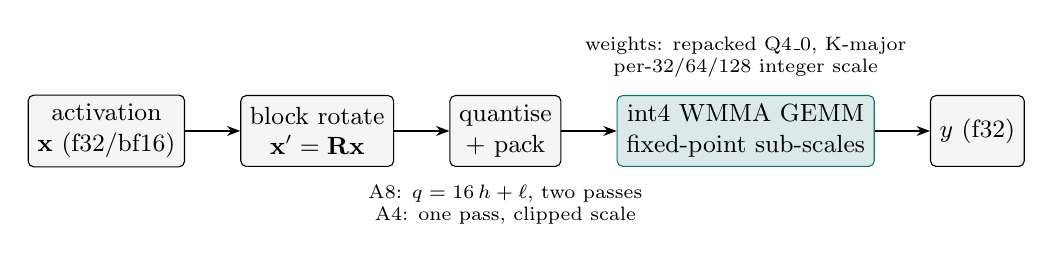
\begin{tikzpicture}[node distance=7mm,>=Stealth,
  box/.style={draw,rounded corners=2pt,minimum height=9mm,align=center,font=\small,fill=black!4},
  hot/.style={box,fill=cgood!15,draw=cgood}]
\node[box] (x) {activation\\$\X$ (f32/bf16)};
\node[box,right=of x] (r) {block rotate\\$\X'=\HD\X$};
\node[box,right=of r] (q) {quantise\\+ pack};
\node[hot,right=of q] (g) {int4 WMMA GEMM\\fixed-point sub-scales};
\node[box,right=of g] (y) {$y$ (f32)};
\draw[->] (x)--(r); \draw[->] (r)--(q); \draw[->] (q)--(g); \draw[->] (g)--(y);
\node[font=\scriptsize,below=1mm of q,align=center] {A8: $q=16\,h+\ell$, two passes\\A4: one pass, clipped scale};
\node[font=\scriptsize,above=1mm of g,align=center] {weights: repacked Q4\_0, K-major\\per-32/64/128 integer scale};
\end{tikzpicture}
\caption{Prefill GEMM pipeline for a rotated tensor (rotate, quantise and pack are one fused kernel).}
\end{figure}

\subsection{Eight-bit activations on int4 hardware (default prefill, ``quality'')}
Every int8 code $q\in[-128,127]$ is split as $q=16h+\ell$ with $h\in[-8,7]$ signed and $\ell\in[0,15]$ unsigned. The GEMM
runs the $h$ pass, shifts the integer accumulator by 4 bits, runs the $\ell$ pass into the \emph{same} accumulator, and then
applies the integer weight sub-scale. Two int4 passes cost the same as one int8 pass, but the iu4 pipe is the one that is twice
as fast, so the effective rate is 134 int4-TOPS $=$ 67 int8-equivalent TOPS (about 74\% of the iu4 ceiling) against 36--40 TOPS
for the stock INT8 MMQ path. Integer weight scales use a fixed-point shift (SH8 $=12$), and the final cross-unit accumulation is
carried in float to avoid 24-bit overflow in the integer multiply-adds.

The weight scale group is detected at load time (\tx{k_detect_gw}: GW $\in\{1,2,4\}$ means 32/64/128 columns per scale), so
the same kernel serves group-32, 64 and 128 files; group~64 gives about +5\% prefill for KLD 0.029 (0.0228 at group 32 with
the Q8 head), group 128 would be about KLD 0.04.

\subsection{Four-bit activations (the ``fast'' path)}
A single int4 pass, with the activation scale per 256-block expressed as a multiplier $m\in\{1,\ldots,16\}$ of $1/16$ of a
per-token reference scale: $m_b=\lceil 16\,\mathrm{clip}\cdot\mathrm{amax}_b/\mathrm{amax}_{\text{token}}\rceil$ (this mirrors the
simulation's \tx{act_quant}). Weight scales use SH $=10$. The \textbf{clip} factor shrinks the quantiser range so rare outliers
saturate instead of stretching the scale:

\begin{figure}[H]
\centering\includegraphics[width=.55\linewidth]{fig/clip.pdf}
\caption{Effect of the 4-bit activation clip (all tensors A4; KLD vs BF16). The default 0.85 reduced KLD from 0.113 to 0.092
at no cost in speed; 0.6 is too aggressive.}
\label{fig:clip}
\end{figure}

\subsection{Choosing activation width per tensor kind}
Environment variables select which tensors take the 4-bit path; everything else stays at 8 bit.
\begin{table}[H]
\centering\small
\caption{Control surface of the INT4 backend.}
\begin{tabularx}{\linewidth}{@{}lX@{}}
\toprule
Variable & Meaning\\
\midrule
\tx{GGML_INT4=1/2/3} & 1: rotation only; 2: 4-bit activations everywhere; 3: 8-bit activations (auto-set by the loader for rotated files)\\
\tx{GGML_INT4_PREFILL} & \tx{quality} (default): no A4; \tx{balanced}: A4 on \txl{attn_q.weight,attn_k,attn_v,attn_qkv,attn_gate,ffn_gate,ffn_up}; \tx{fast}: A4 on \tx{attn_,ffn_,ssm_}\\
\tx{GGML_INT4_A4=<substrings>} & explicit list of tensor-name substrings that use A4 (overrides the preset)\\
\tx{GGML_INT4_CLIP} & 4-bit activation clip factor, default 0.85\\
\bottomrule
\end{tabularx}
\end{table}

Per-kind sensitivity (simulation with GPTQ weights; baseline KLD 0.0269; Figure~\ref{fig:kinds}) shows why one cannot rescue
speed with a clever per-layer mix: the FFN has the FLOPs \emph{and} the sensitivity.

\begin{figure}[H]
\centering\includegraphics[width=.8\linewidth]{fig/kinds.pdf}
\caption{Added KLD when one tensor kind alone moves to 4-bit activations. FFN down/up/gate and the GDN out-projection dominate.}
\label{fig:kinds}
\end{figure}

%=====================================================================================================================
\section{Decode: from 92 to 132 tokens/s}
\label{sec:decode}

The first working INT4 path decoded at only 91.9\,t/s with the older RTN file. Diagnosis and fixes:
\begin{itemize}
\item \textbf{Decode is launch-bound, not bandwidth-bound.} The GPU is about 64\% busy with $\sim$3\,\textmu s gaps between
      $\sim$620 kernels per token; the matvec kernels already stream at the $\sim$733\,GB/s ceiling. So the lever is fewer and
      leaner kernels, not faster matvecs.
\item \textbf{Keep CUDA graphs and matmul fusion enabled.} The INT4 hook had disabled them; they are now skipped only for a rotated
      weight that cannot take the fused path (\txl{ggml_cuda_int4_fused_ok}).
\item \textbf{Fuse the rotation into Q8\_1 quantisation} for batches $\le 8$ (\tx{k_rot_q8_1}, called from \txl{mul_mat_vec_q}):
      one kernel instead of rotate-then-quantise. Decode always uses 8-bit activations, so it carries no A4 penalty.
\item \textbf{Shrink the head.} The 1.27\,GB BF16 tied embedding/head cost about 1\,ms per token alone. Q6\_K costs +0.002 KLD and
      buys +6 t/s; Q8\_0 is KLD-better (0.0228) but slower (126.6 t/s).
\end{itemize}
Result: 132.6 t/s (Q6\_K head) / 126.6 t/s (Q8\_0 head), against 131.6 t/s for Q4\_K\_M. All preset changes later in the work left
tg128 within 130--132.

%=====================================================================================================================
\section{Results: Q4-quality at higher prefill}
\label{sec:q4}

Median of 8 runs after the first; KLD on 24 chunks of WikiText-2 test; MMAU with the audio patch.

\begin{table}[H]
\centering\small
\caption{Rotated-INT4 files vs Q4\_K\_M (RX 7900 XT, ROCm 10.1.0, 8-bit prefill activations).}
\begin{tabular}{@{}lrrrrrrrr@{}}
\toprule
Model & GB & pp512 & pp2048 & tg128 & PPL vs BF16 & KLD & top-1 & MMAU\\
\midrule
Q4\_K\_M & 2.7 & 4{,}733 & 4{,}595 & 131.6 & +3.3\% & 0.032 & 91\% & 72.2\\
rotq4-gptq (Q6\_K head) & 2.55 & \textbf{5{,}571} & \textbf{5{,}399} & \textbf{132.6} & +1.9\% & 0.0246 & 92.2\% & 71.7\\
rotq4-gptq-q8head & 2.70 & 5{,}622 & 5{,}402 & 126.6 & +1.7\% & 0.0228 & 93.5\% & 72.0\\
\emph{older:} rotq4g4 (RTN, A4) & 3.3 & 8{,}041 & 7{,}615 & 91.9 & +17.6\% & 0.197 & 81\% & 69.0\\
\bottomrule
\end{tabular}
\end{table}
So the answer to ``get it to Q4 quality'' is positive: prefill $+18\%$ at that point, decode at par, and KLD \emph{below}
Q4\_K\_M's (0.023--0.025 vs 0.032), with MMAU inside noise of Q4\_K\_M and BF16.
The group-64 variant with the Q8 head gave KLD 0.0293 (so group-32 stays the default).
Note that 0.0246 above is from before the wave32 GDN kernel of Section~\ref{sec:gdn}; the same file measures 0.0252 after it
(floating-point summation order changes; the difference is inside the $\pm$0.0012 standard error).

%=====================================================================================================================
\section{Reaching 8k prefill}
\label{sec:8k}

The target: pp512 $\approx$ 8{,}000 tokens/s with decode held at $\sim$132 t/s. The 8-bit GEMM pair of passes is itself
close to its ceiling (Section~\ref{sec:tile}), so the remaining levers were (a)~use fewer GEMM bits per tensor, (b)~speed up
the non-GEMM parts (gated-delta-net recurrence first), (c)~recover the quality of (a).

\subsection{Per-kind A4 sweep}
\tx{scripts/sweep_a4.sh} runs, for each activation-width configuration of the \emph{same} GGUF, KLD (24 chunks) and
the median bench. Results (Figure~\ref{fig:pareto} plots them against the standard quants):

\begin{table}[H]
\centering\small
\caption{Prefill preset sweep on \protect\txl{ossicle-4b-gptq-g32-q6e.gguf}. Tokens/s are medians; ``A4 on'' lists the tensor kinds using
single-pass 4-bit activations (clip 0.85); the rest are A8.}
\label{tab:sweep}
\begin{tabular}{@{}lrrrrr@{}}
\toprule
A4 on & pp512 & pp2048 & tg128 & KLD & top-1 \%\\
\midrule
nothing (\tx{quality}) & 5{,}846 & 5{,}647 & 131.8 & 0.0252 & 92.5\\
q/k/v, qkv, z-gate, ffn gate & 6{,}784 & 6{,}488 & 131.9 & 0.0519 & 89.3\\
\;+ ffn up (\tx{balanced}) & 7{,}257 & 6{,}935 & 131.5 & 0.0713 & 87.3\\
\;+ ffn down & 7{,}857 & 7{,}504 & 131.3 & 0.0871 & 86.8\\
everything (\tx{fast}) & \textbf{8{,}248} & 7{,}797 & 131.9 & 0.0964 & 85.4\\
\bottomrule
\end{tabular}
\end{table}

\begin{figure}[H]
\centering\includegraphics[width=.9\linewidth]{fig/pareto.pdf}
\caption{Prefill speed against fidelity. Stock quants cluster at 4.0--4.8k t/s; the rotated-INT4 sweep moves right along a roughly
linear speed--KLD trade-off from 5.8k to 8.2k. (Stock KLD from the full-study table; INT4 points from the sweep above.)}
\label{fig:pareto}
\end{figure}

The final confirmation run of \tx{fast} on the committed build gave pp512 8{,}269 / pp2048 7{,}802 / tg128 131.7 (the sweep run
measured 8{,}248 / 7{,}797 / 131.9; run-to-run variation is $\sim$0.3\%). Likewise the \tx{balanced} confirmation gave
pp512 7{,}243 / pp2048 6{,}930 against the sweep's 7{,}257 / 6{,}935. We quote the final numbers in the abstract and the sweep
numbers in this table; neither is a transcription error.

\begin{table}[H]
\centering\small
\caption{Final presets, same file (\tx{rotq4-gptq}, Q6\_K head).}
\begin{tabular}{@{}lrrrrrrr@{}}
\toprule
Preset & pp512 & pp2048 & tg128 & PPL vs BF16 & KLD & top-1 & MMAU\\
\midrule
\tx{quality} (A8 everywhere) & 5{,}846 & 5{,}647 & 131.8 & +1.9\% & 0.0252 & 92.5\% & 71.7\\
\tx{balanced} & 7{,}243 & 6{,}930 & 131.1 & -- & 0.071 & 87.3\% & --\\
\tx{fast} (A4 everywhere) & \textbf{8{,}269} & \textbf{7{,}802} & \textbf{131.7} & +7.4\% & 0.096 & 85.4\% & 71.6\\
\bottomrule
\end{tabular}
\end{table}

\paragraph{Reading the trade-off.} \tx{fast} sits between Q4\_0 (KLD 0.058) and Q3\_K\_L (0.101) on KLD at about twice the
Q3 prefill rate. Its MMAU score (71.6) is indistinguishable from \tx{quality} (71.7), but MMAU has $\pm1.4$\,pp noise and
audio questions are dominated by the audio encoder; the KLD/PPL numbers are the more sensitive indicators and they do degrade.
Four-bit activations carry about 10\% relative noise per matmul (20\,dB SNR); at 8k the KLD cannot be recovered without
more bits.

\subsection{Where the speed comes from}
\begin{itemize}
\item \textbf{GEMM bit-width}: one pass instead of two for A4 tensors (the bulk of the 5{,}846\,$\to$\,8{,}269 gain).
\item \textbf{Activation clip 0.85}: quality only (KLD 0.113\,$\to$\,0.092 in the clip experiment), no speed effect.
\item \textbf{Wave32 gated-delta-net kernel}: $+5\%$ prefill (5{,}571\,$\to$\,5{,}846 at pp512), Section~\ref{sec:gdn}.
\end{itemize}

\subsection{Tile shapes}
\label{sec:tile}
The GEMM tile constants (MI$=$2, NJ$=$2, WAVES\_N$=$8) were varied: (2,2,4), (2,2,16) and (1,2,8) all landed within 2\% of
each other. The prefill GEMM is therefore near its practical ceiling (about 74\% of iu4 peak at A8), and the rest of the
prefill budget is no longer the GEMM alone: at \tx{fast}, a 512-token pass takes $\approx$62\,ms of which gated-delta-net is
22\%, flash attention 3--7\%, and rotate+quantise $\approx$3\%.

%=====================================================================================================================
\section{Gated-delta-net: what worked and what did not}
\label{sec:gdn}

The recurrence per head is $S_t = a_t\,S_{t-1} + k_t\,\delta_t^{\!\top}$ with $\delta_t = \beta_t\,(v_t - S_{t-1}^{\!\top}k_t)$ and
output $o_t=S_t^{\!\top}q_t$; state $S\in\mathbb{R}^{128\times128}$ per head, 24 GDN layers, 32 value heads. It is
sequential in $t$, and at pp512 it takes 0.54\,ms per layer per 512 tokens (22\% of a \tx{fast} pass).

\subsection{Kept: two lanes per state column (wave32)}
\tx{gated_delta_net_cols} (HIP only, $S_v{=}128$, scalar gate, non-KDA): each state column is owned by \emph{two} lanes holding
64 state registers each; one \texttt{\_\_shfl\_xor(\ldots,16)} per reduction; $k$/$q$ double-buffered in wave-private LDS; the next token's
$v,\beta,g$ prefetched. Grid $(H, n_{\text{seqs}}, 2)$, block $(32,4)$. Gain: +5\% prefill (pp512 5{,}571\,$\to$\,5{,}846), KLD unchanged
within error. The path that led here:
\begin{itemize}
\item Software pipelining of the original kernel's loads: no gain.
\item One lane per column: 256 VGPRs, spilled. LDS-staged variant: worse. \emph{Two} lanes per column (64 state registers each): fixed it.
\item Prefetching $v,\beta,g$ in the new kernel: no measurable gain.
\end{itemize}

\subsection{Reverted: chunked WY form}
The chunked form turns the recurrence into matrix products per chunk of $C$ tokens: build the strictly lower-triangular
interaction $L$, invert $(I+L)$, form $\eta=U-W S_0$, produce the chunk's outputs, and update the state. We implemented a prep
kernel and a scan kernel; both were \emph{correct} (KLD 0.0249 against 0.0252 for the recurrent kernel) but slower:
\begin{center}\small
\begin{tabular}{@{}lr@{}}
\toprule
Variant & pp512 (A8 mode)\\
\midrule
recurrent \tx{cols} kernel (kept) & \textbf{5{,}846}\\
chunked, $C{=}64$ (spills; one \texttt{waitcnt} per LDS load) & 3{,}401\\
chunked, $C{=}32$, rolled loops & 5{,}307\\
chunked, final restructure (scan spills 1{,}988\,B scratch) & 4{,}674\\
\bottomrule
\end{tabular}
\end{center}
Without matrix instructions the chunk algebra is bound by LDS latency and register pressure on RDNA3. The work was reverted
with \tx{git checkout} and saved as \txl{kernel/gated_delta_net_chunked_wip.cu} (also uploaded). The follow-up is a WMMA-based
chunk kernel; at 22\% of a pass, even a free GDN would give $\sim$+28\% on \tx{fast} and would let a middle preset reach
8k at higher fidelity.

%=====================================================================================================================
\section{Negative and neutral results (consolidated)}
\label{sec:neg}

\begin{center}\small
\begin{tabularx}{\linewidth}{@{}>{\raggedright\arraybackslash}p{3.6cm}X@{}}
\toprule
Idea & Outcome\\
\midrule
RTN rotated int4 + A4 (first integrated file) & KLD 0.197--0.220; usable speed (8{,}041 pp512) but PPL +17.6\%; superseded.\\
Wider weight scale groups (64/128) & +5\% prefill for +0.005--0.015 KLD; group 32 kept as default.\\
NVFP4/MXFP4 $\to$ uniform int4 & +0.07 KLD, no gain over BF16$\to$int4.\\
Sparsity skipping in the GEMM & Exact and fast on synthetic sparsity; real tiles are 0--6\% skippable.\\
Tile-shape retuning (MI,NJ,waves) & Flat within 2\%.\\
Per-layer A4/A8 mix without per-kind logic & FFN carries both FLOPs and sensitivity; no mix recovers 8k at A8 quality.\\
GDN software pipelining; LDS-staged cols; v/$\beta$/g prefetch & No gain or worse.\\
Chunked WY GDN (scalar code) & Correct but 9--42\% slower than recurrent (above).\\
Clip 0.6 for A4 & KLD 0.146, worse than no clip (0.113); 0.7: 0.093; 0.85 chosen (0.092).\\
\bottomrule
\end{tabularx}
\end{center}

\section{Failures and mishaps during the run}
\label{sec:errors}
\begin{itemize}
\item \textbf{Disk exhaustion.} Both filesystems ran full. \tx{/mnt/data} was at 1.4\,GB free, so GPTQ safetensors were written to
      \txl{/home/svt/ossicle-tmp}; intermediates and old GGUFs were deleted as needed; the group-128 GPTQ run failed with ENOSPC and
      was dropped.
\item \tx{__builtin_amdgcn_wmma_*} requires constant flags; a runtime \tx{pass == 0} flag failed to compile and was replaced by
      separate if/else branches.
\item A calibration file deleted while a simulation was starting broke one sweep; it was re-run on \txl{wiki.train.raw}.
\item \txl{llvm-objdump --offloading} scattered extracted bundle files into the build \tx{bin} directory; removed with a targeted \tx{rm}.
\item A \tx{pkill -f} pattern matched and killed the controlling shell; replaced by explicit PIDs. A relative-glob \tx{rm} was blocked
      by the safety check and a fresh directory was used instead.
\item The harness blocked \tx{sleep} chained to \tx{tail}; polling loops of \tx{grep -q} with short sleeps were used instead.
\end{itemize}

%=====================================================================================================================
\section{Caveats and limitations}
\label{sec:caveats}
\begin{itemize}
\item \textbf{RDNA3 only} (gfx1100 family, ROCm). The GGUFs are \emph{not} ordinary Q4\_0 files: any other build or backend
      decodes the rotated codes as if they were unrotated and produces garbage. They only work with the \tx{ossicle} branch.
\item \textbf{Detection heuristic:} any \tx{blk.*} Q4\_0 tensor with $K \bmod 256=0$ is treated as rotated when
      \txl{ossicle.int4_rotation_block} is present.
\item \textbf{VRAM:} a repacked copy of each weight is kept next to the Q4\_0 tensor, roughly doubling weight VRAM.
\item \textbf{Integer headroom:} the 24-bit integer multiply-adds assume activation sums that fit 24 bits. True for real data with
      about 8$\times$ margin at 8-bit; not guaranteed for adversarial inputs.
\item \textbf{Calibration is text-only} (WikiText-2 train); the audio path is not represented, and MMAU ($\pm$1.4\,pp)
      is too coarse to detect a loss of the size KLD shows.
\item \textbf{Single GPU, no MoE, no batched matmul;} one run per MMAU configuration; KLD from 24 chunks.
\item \textbf{Unexplained 0.005 KLD difference:} the all-A4 clip experiment (\tx{GGML_INT4=2}, clip 0.85) gave KLD 0.0917, while the
      \tx{fast} preset (per-tensor A4 list covering everything) gives 0.0964. We did not chase it down; plausible causes are
      per-tensor fixed-point shift selection in the preset path, or the preset's tensor list not matching the mode-2 set exactly.
\item \textbf{Licence:} the HF repository's licence field is still \tx{other}; set a real licence before making it public.
\item The HF repo (\txl{SILVERTHRONE/Ossicle-4B-GGUF}) and the GitHub fork are \emph{private}.
\end{itemize}

%=====================================================================================================================
\section{Reproduction}
\label{sec:repro}

\paragraph{Build the INT4 file.}
\begin{lstlisting}[language=bash]
# 1. BF16 GGUF from the safetensors
python scripts/convert_ossicle.py  ...                      # -> ossicle-4b-bf16.gguf

# 2. GPTQ on rotated weights (needs HF safetensors, ~15 GB RAM, ~4 min, writes ~2.5 GB)
python scripts/gptq_rotate.py --src stage_lm --out gptq_g32.safetensors --group 32 --calib 128

# 3. Rebuild the GGUF from BF16 with the GPTQ blocks; Q6_K head; per-tensor error check
python scripts/rotate_quantize.py ossicle-4b-bf16.gguf ossicle-4b-gptq-g32-q6e.gguf \
       --blocks gptq_g32.safetensors --embd q6_k
\end{lstlisting}

\paragraph{Run it.}
\begin{lstlisting}[language=bash]
GGML_INT4_PREFILL=fast llama-server -m rdna3/ossicle-4b-rotq4-gptq.gguf \
    --mmproj mmproj-ossicle-4b-f16.gguf --jinja -ngl 99          # drop the variable for the quality default
\end{lstlisting}

\paragraph{Measure it.}
\begin{lstlisting}[language=bash]
# KLD (24 chunks vs the BF16 base logits) + full bench for one configuration
scripts/measure_int4.sh <tag> <model.gguf> GGML_INT4=3 GGML_INT4_PREFILL=fast
#   = llama-perplexity -m M -f wiki.test.raw -c 512 -ngl 99 --chunks 24 \
#                      --kl-divergence-base kld_base.bin --kl-divergence

# median of 8 runs (llama-bench -p 512,2048 -n 128 -r 9, first sample dropped)
scripts/bench_med.sh <model.gguf> GGML_INT4_PREFILL=fast

# per-kind A4 sweep
scripts/sweep_a4.sh <model.gguf> out.tsv "none:none" "fast:attn_,ffn_,ssm_" ...

# MMAU test-mini via llama-server (with the audio patch's mmproj)
scripts/run_mmau_int4.sh  [EXTRA=env]

# Simulation behind Figure 1 (HF transformers, needs GPU)
python int4/w4a4_sim2.py --calib 128 --configs "fp16" "wg=32,wm=gptq,a=8" "wg=32,wm=gptq,a=4" ...
\end{lstlisting}

\section{Artefacts}
\begin{itemize}
\item \textbf{Fork:} \txl{github.com/SILVERTHRONE32/llama.cpp-ossicle}, branch \tx{ossicle}, head \tx{1fcc55e87}. Commit stack on
      top of upstream \tx{f2b52a87e}: \tx{0fc5f77a2} (audio keys), \tx{22ca9a167} (opt-in INT4 WMMA prefill), \tx{fe6ca0637} (8-bit
      activations, graphs/fusion kept), \tx{2b78d7055} (rotation fused into Q8\_1, GW-chained kernel, group auto-detect),
      \tx{2d6f34eee} (loader auto-enable), \tx{1fcc55e87} (presets, clip, wave32 GDN). Diff against the audio base: six files,
      +969/$-$1 lines (\tx{int4-wmma.cu} 779 lines, \txl{gated_delta_net.cu} +121, \tx{ggml-cuda.cu} +36, \tx{mmvq.cu},
      \tx{int4-wmma.cuh}, \txl{llama-model-loader.cpp}).
\item \textbf{HF repo (private):} \txl{SILVERTHRONE/Ossicle-4B-GGUF}: \txl{rdna3/ossicle-4b-rotq4-gptq.gguf} (2.55\,GB),
      \txl{rdna3/ossicle-4b-rotq4-gptq-q8head.gguf} (2.70\,GB), \txl{experimental/ossicle-4b-rotq4g4.gguf} (older RTN),
      the ten standard quants, mmproj, model card, patches (\txl{llama.cpp-ossicle-audio.patch}, \txl{llama.cpp-ossicle-int4.patch}),
      scripts, \txl{int4/w4a4_sim2.py}, and the chunked GDN WIP kernel.
\item \textbf{Local:} \txl{/mnt/data/projects/ossicle-gguf} (scripts, logs in \tx{work/}, kernels in \tx{kernel/}, simulations in \tx{int4/}),
      main model \txl{/home/svt/ossicle-tmp/ossicle-4b-gptq-g32-q6e.gguf}.
\end{itemize}

\section{Next steps}
\begin{enumerate}
\item \textbf{Default preset.} Decide whether \tx{fast} should be the default for rotated files, or keep \tx{quality} and document
      \tx{fast} as opt-in (current state).
\item \textbf{WMMA chunked GDN.} A tensor-core chunk kernel is the one lever that raises speed \emph{without} costing KLD, and
      is what would make 8k reachable at \tx{balanced}/\tx{quality} fidelity.
\item \textbf{Close the 0.005 KLD gap} between the mode-2 clip experiment and the \tx{fast} preset.
\item \textbf{Audio-aware calibration} for GPTQ (mix speech/sound/music features into the Hessian text), and a larger MMAU sample or
      multiple seeds to resolve differences below $\sim$2\,pp.
\item Set a licence and decide on public release of the HF repository.
\end{enumerate}

\end{document}
